% Reaaliaikainen renderöinti -kurssin harjoitustyö

\documentclass[utf8,bachelor]{gradu3}
\usepackage[bookmarksopen,bookmarksnumbered,linktocpage]{hyperref}
\usepackage{mathtools}
\usepackage{graphicx} % kuvia varten
\usepackage{amssymb} % lukujoukkojen symbolit. Käyttöesim. $\mathbb{set}$
\usepackage{amsmath} % overbrace, underbrace
\DeclareMathOperator{\sgn}{sgn}
\addbibresource{StarwWeaveShader.bib}


%% ##############################
\begin{document}

\title{Punosvarjostin}

\translatedtitle{Straw weave shader}

%\studyline{}
\avainsanat{avain1, avain2, avain3}
\keywords{avainsanat englanniksi}
\tiivistelma{Tiivistelmä on tyypillisesti 5-10 riviä pitkä esitys työn pääkohdista (tausta, tavoite, tulokset, johtopäätökset).
}
\abstract{Englanninkielinen versio tiivistelmästä.
}

\author{Kimmo Riihiaho}
\contactinformation{\texttt{kimmo.a.riihiaho@student.jyu.fi}}
% jos useita tekijöitä, anna useampi \author-komento
\supervisor{Jarno Kansanaho}
% jos useita ohjaajia, anna useampi \supervisor-komento
\type{} % tämän makron oletus on ''pro gradu -tutkielma'' ja bachelor-optiolla kandidaatintutkielma

\maketitle

\mainmatter

\chapter{Idea}

Tarkoituksena on luoda varjostinohjelma, jolla voi kuvata punosta. Alunperin ajatuksena oli kuvata olkipunosta, mutta varjostin soveltunee myös esim. kankaan kuvaamiseen. Punoksen kuvaaminen $x-y$-tasossa on suhteellisen yksinkertaista, mutta jotta sitä voisi käyttää kaareville pinnoille, tarvitaan koordinaattimuunnoksia varten malliavaruuden lisäksi pinnan paikallinen normaali - luulisin.

Tavoitteena olisi saada varjostin toimimaan edes yhteen suuntaan kaareutuvalle pinnalle.  

Olen toteuttanut punoksen Blenderin Cycles-renderöijän node-ohjelmoinnilla kuvaamaan tatamin pintaa, joka näkyy kuvassa \ref{fig:room}. Käytin samaa tekstuuria suuremmalla skaalauksella myös kuvassa näkyvään patjaan.

\begin{figure}[h] 
	\centering
	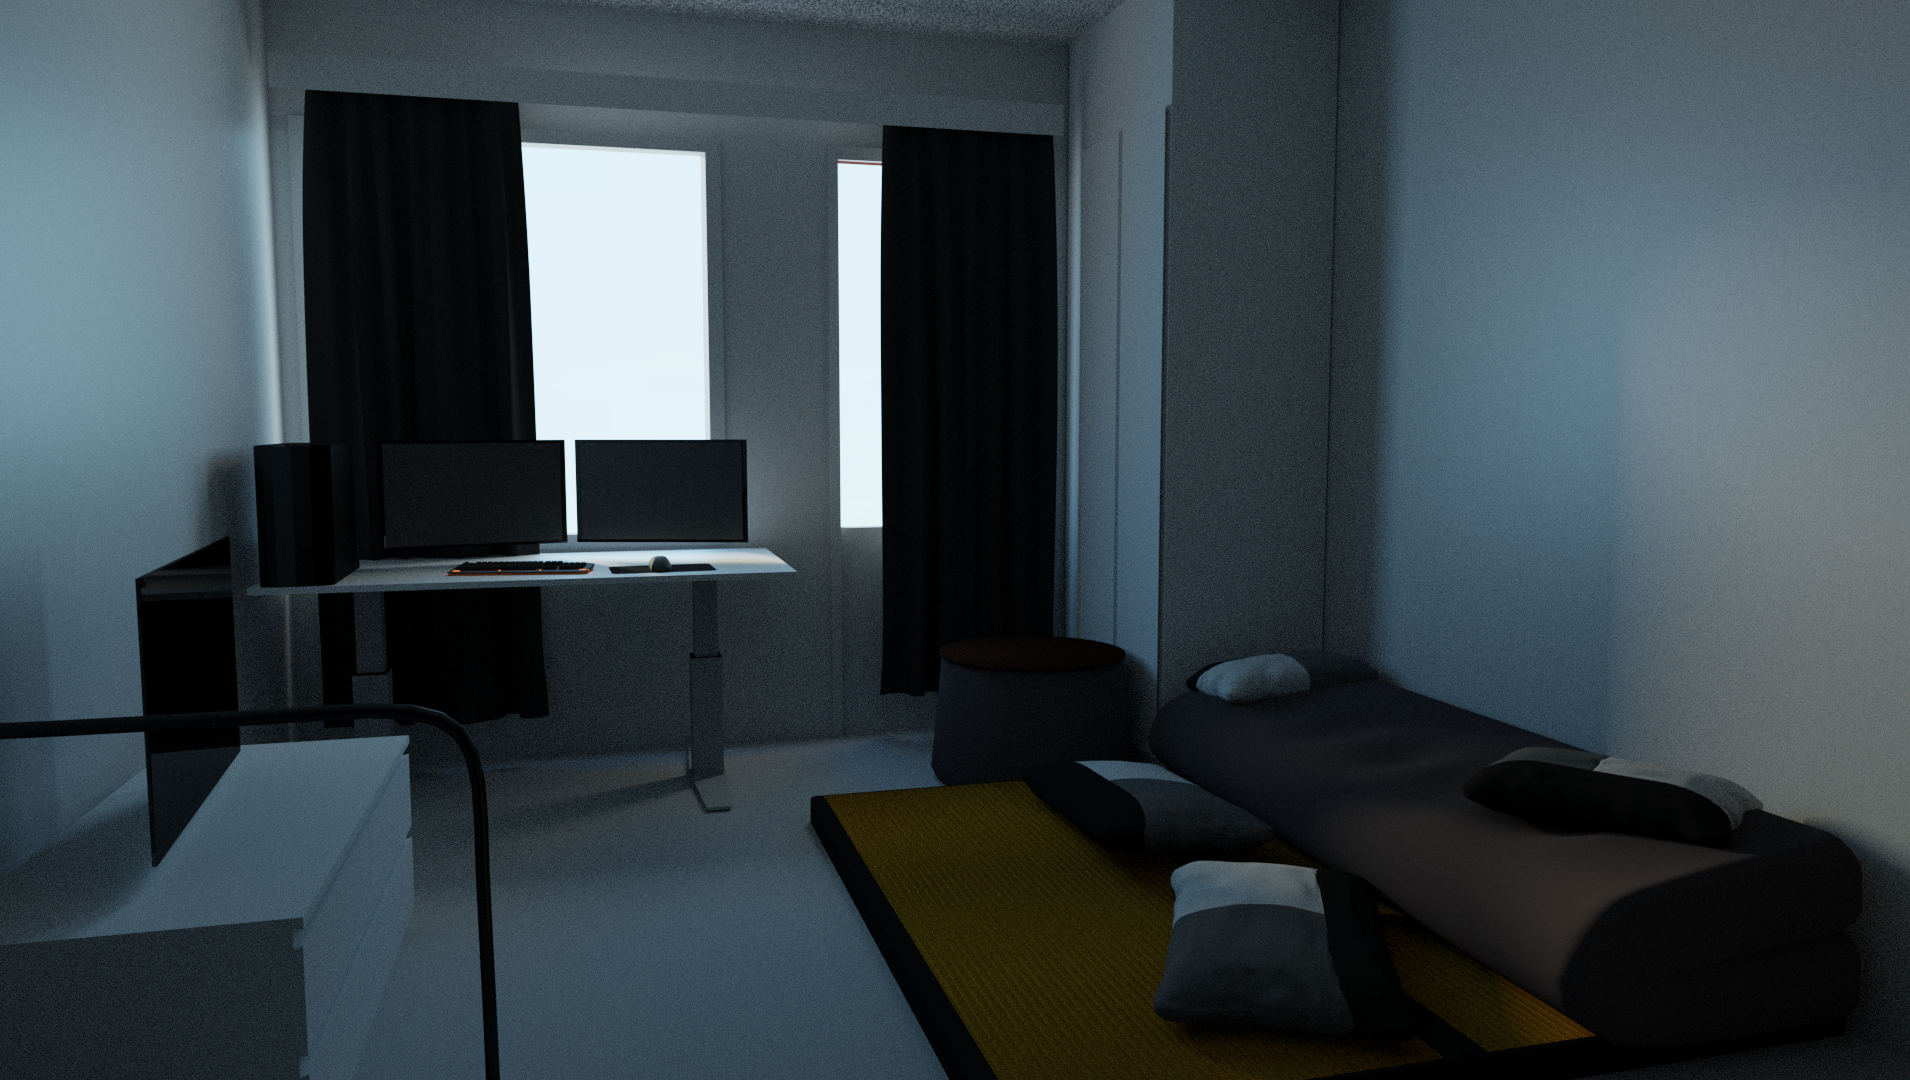
\includegraphics[height=8cm]{day1.png}
	\caption{Blenderillä mallinnettu huone, jossa on käytetty proseduraalista punostekstuuria.}
	\label{fig:room}
\end{figure}

\chapter{Matemaattinen perusta}

Yksinkertaisen punosta kuvaavan funktion saa kohtalaisella vaivalla määriteltyä $x-y$-tasoon. Määritellään aluksi skaalausfunktio $f_a$ $x$-akselin suuntaan.

\begin{equation}
\label{eq:warp}
f_a(x) = \frac{xs_o}{s_a} = a,
\end{equation}

jossa $s_o$ on yleisskaalaus, $s_a$ on loimen suuntainen skaalaus ja $x$ on malliavaruuden $x$-koordinaatti. Alaindeksillä $a$ tarkoitetaan loimeen (engl. warp) liittyviä asioita. Loimiskaalauksen $s_a$ kasvaessa loimilangat siirtyvät kauemmaksi toisistaan ja punos loivenee. Yleisskaalauksen $s_o$ (engl. overall) kasvaessa koko punos skaalautuu pienemmäksi.

Vastaavasti määritellään $y$-akselin suuntaan skaalaava funktio $f_e$

\begin{equation}
\label{eq:weft}
f_e(y) = \frac{ys_o}{s_e} = e,
\end{equation}

jossa $s_e$ on kudelangan (engl. weft) leveys.

Seuraavaksi määritellään funktio $f_c$ kuvaamaan kudelangan pyöreyttä

\begin{equation}
\label{eq:curvature}
f_c(e) = r\lvert\sin{e}\rvert,
\end{equation}

jossa kerroin $r$ määrää pyöristyksen voimakkuuden. $r$:n arvolla $0$ saadaan tuotettua kulmikas kude.

Funktio $f_b$ kuvaa kanttiaaltoa (engl. box), jota käytetään vuorottelemaan vierekkäisiä siniaaltoja, jotta ne näyttäisivät erillisiltä kudelangoilta

\begin{equation}
\label{eq:box}
f_b(e) = \pi \lfloor \sin{e} \rfloor.
\end{equation}

Käyttämällä funktioita~\eqref{eq:curvature} ja~\eqref{eq:box} saadaan punoksen yhtälö $f_w$ $a$:n ja $e$:n suhteen 

\begin{equation*} 
\label{eq:weave_ae}
f_w(a,e) = \sin{\big(a + f_b(e)\big)} + f_c(e),
\end{equation*}

joka laajennetaan $x$:n ja $y$:n suhteen syöttämällä sisään yhtälöt~\eqref{eq:warp},~\eqref{eq:weft},~\eqref{eq:curvature} ja~\eqref{eq:box}

\begin{equation}
\label{eq:weave_xy}
f_w(x,y) = \sin{\big(\frac{xs_o}{s_a} + \pi \lfloor \sin{\frac{ys_o}{s_e}} \rfloor\big)} + r\lvert\sin{\frac{ys_o}{s_e}}\rvert : \mathbb{R}^2 \rightarrow \mathbb{R}.
\end{equation}

Yhtälö \ref{eq:weave_xy} on määritelty koko $\mathbb{R}^2$:ssa, mutta itseisarvo- ja lattiafunkitoiden takia se ei ole jatkuva. 

Lopuksi normalisoidaan yhtälö min-max -skaalauksella~\parencite{dmSlides5} välille $\left[0,1\right]$, jotta kun sitä käytetään pinnan normaalina, se ei painu negatiiviseksi.

\begin{equation}
\label{eq:weave_norm}
f_{wn} = \frac{f_w-\min{(f_w)}}{\max{(f_w)}-\min{(f_w)}} : \mathbb{R}^2 \rightarrow \mathbb{R}.
\end{equation}

Funktion $f_{wn}$ Maxima-plottaus kuvassa \ref{fig:maxima_scale} näyttää skaalausten ja pyöristyksen vaikutuskohdat. 

\begin{figure}[h] 
	\centering
	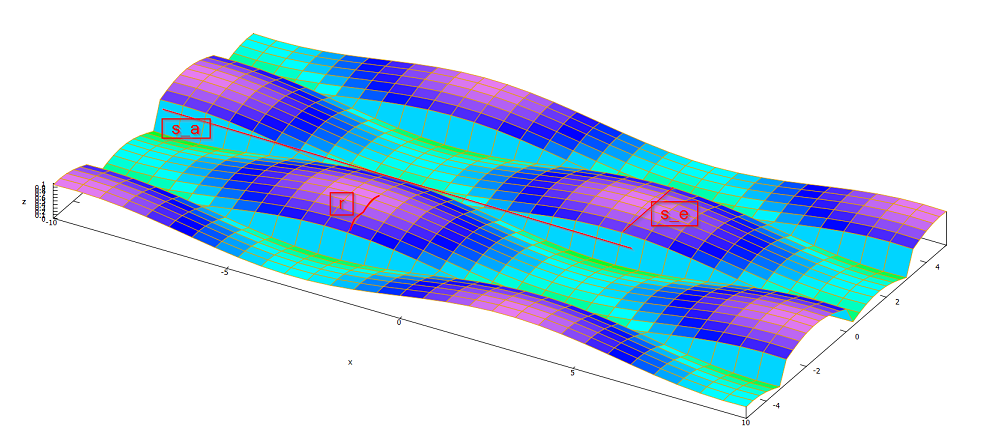
\includegraphics[height=7cm]{weave_plot_scales_maxima_small.png}
	\caption{Skaalausten ja pyöristyksen vaikutus funktion käyttäytymiseen.}
	\label{fig:maxima_scale}
\end{figure}

Jotta funktiota voi käyttää normaalimäppäykseen, pitää laskea funktion normaali pisteessä $(a,e)$ osittaisderivaatan avulla. Yhtälön~\ref{eq:weave_xy} osittaisderivointi $a$:n suhteen on yksinkertaista:

\begin{equation}
\label{eq:partialA}
\frac{\partial f_w(a,e)}{\partial a} = cos(a + \pi\lfloor \sin{e} \rfloor )
\end{equation}

Osittaisderivaatta $e$:n suhteen vaatii lattiafunktion derivoinnin, mikä aiheuttaa pieniä hankaluuksia, sillä lattiafunktio ei ole jatkuva. Lattiafunktion $\lfloor x \rfloor $ derivaatta ei ole määritelty, kun $ x \in \mathbb{N}$, ja kaikkialla muualla se on $0$, joten käytännön tarkoituksessa voimme pitää sitä aina nollana. Itseisarvofunktion $\lvert x \rvert$ derivaatta on $\sgn(x)$, kun $x \neq 0$.

\begin{equation}
\label{eq:partialE}
\begin{aligned}
\frac{\partial f_w(a,e)}{\partial e} & = cos(a + \pi\lfloor \sin{e} \rfloor )  \overbrace{ D \lfloor \sin{e} \rfloor }^\text{= 0} + r \cdot \sgn ( \sin e )\cos e \\
& = r \cdot \sgn ( \sin e )\cos e
\end{aligned}
\end{equation}

Lopullinen normaalivektori pisteessä $(a,e)$ on tällöin $(\frac{\partial f_w(a,e)}{\partial a}, \frac{\partial f_w(a,e)}{\partial e}, f_w(a,e))$.

\chapter{Käytännön toteutus}

\section{Verteksivarjostin}

Jotta saamme laskettua normaalivektorit muillekin kuin tasasille pinnoille, täytyy käyttää tangenttiavaruutta. Muunnos malliavaruudesta tangenttiavaruuteen lasketaan verteksivarjostimessa jokaiselle verteksille erikseen. Tangenttiavaruus käyttää verteksin normaalia z-suuntana, ja vastaavat x- ja y-suunnat (tangentti ja bitangentti) lasketaan ristitulolla niin, että ensin asetetaan päävektori osoittamaan johonkin suuntaan. Mikäli päävektori on saman suuntainen verteksin normaalin kanssa, päävektori käännetään johonkin muuhun suuntaan.

%Käytännössä asetin päävektorin ensin malliavaruuden x-akselin suuntaiseksi, ja muodostin tangenttiavaruuden sillä. Jos normaa

Jotta siirtymä kolmion reunojen välillä olisi pehmeä, normaali pitäisi interpoloida reunan läheisyydessä, mutta tätä toiminnallisuutta en toteuttanut. Lisäksi x- ja y-koordinaatit pitäisi jatkaa sulavasti reunan yli.

\section{Pikselivarjostin}

Pikselivarjostin laskee pinnan normaalin suunnan käyttäen verteksivarjostimen antamia tangenttiavaruuden arvoja.

Jostain syystä a:n suuntainen osittaisderivaatta näyttää paremmalta, kun termi a jätetään kokonaan pois.

E:n suuntaisen derivaatan vaikutus on hyvin pieni, ja sille voidaan hyvin käyttää arvoa nolla.

\chapter{Ohjelmisto}

Varjostimen testaamista varten kehitetään yksinkertainen kehyssovellus. Kehyssovellus jaetaan alustavasti luokkiin kuvan \ref{fig:ClassDiagram} mukaisesti. Ohjelman karkea rakenne komponenttitasolla on esitetty kuvassa \ref{fig:ComponentDiagram}.

\begin{figure}[h] 
	\centering
	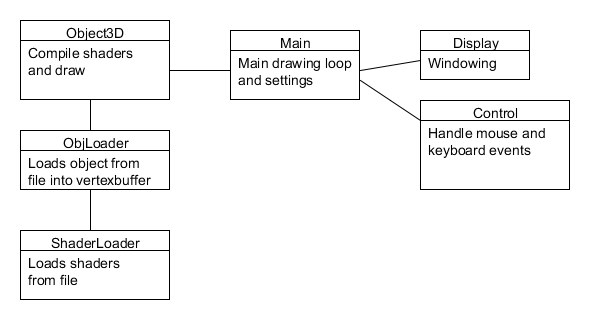
\includegraphics[height=7cm]{ClassDiagram.png}
	\caption{Alustava luokkakaavio.}
	\label{fig:ClassDiagram}
\end{figure}

\begin{figure}[h] 
	\centering
	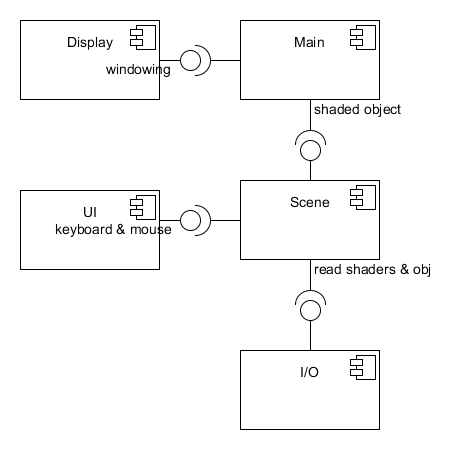
\includegraphics[height=7cm]{ComponentDiagram.png}
	\caption{Alustava komponenttikaavio.}
	\label{fig:ComponentDiagram}
\end{figure}

\printbibliography 

\end{document}
